\documentclass[10pt, a4paper]{article}
\usepackage[a4paper, margin=1.5cm]{geometry}
\usepackage[utf8]{inputenc}
\usepackage[T1]{fontenc}
\usepackage[english]{babel}
\usepackage{lmodern}
\usepackage{amsmath}
\usepackage[center]{caption}
\usepackage{multicol}
\usepackage{graphicx}

\setlength{\parskip}{2pt}
\begin{document}
\begin{center}
    {\Large \textbf{Maciej Kuźmicki --- Multi-View VAE Lab Report}}\\[0.2cm]
    {https://github.com/MaciejKuzmicki/Multi-View-VAE}
    \rule{\textwidth}{0.5pt}
\end{center}

\begin{multicols}{2}
\section*{1. Objective}
The goal of this laboratory was to implement a Multi-View Variational Autoencoder (VAE) capable of learning a shared latent representation from two different image datasets: MNIST and SVHN. The project focused on image reconstruction, generating new samples, and performing cross-domain translation between the two modalities.

\columnbreak

\section*{2. Model Architecture}
The Multi-View VAE uses separate encoders for MNIST (grayscale) and SVHN (RGB). Then, a Mixture of Experts combines them into a shared latent space. Decoders reconstruct the original images. Each domain also has its own encoder and decoder, so the model can generate data even if one view is missing. The idea is shown on figure \ref{fig:architecture}.
\end{multicols}
\begin{figure}[h!]
    \centering
    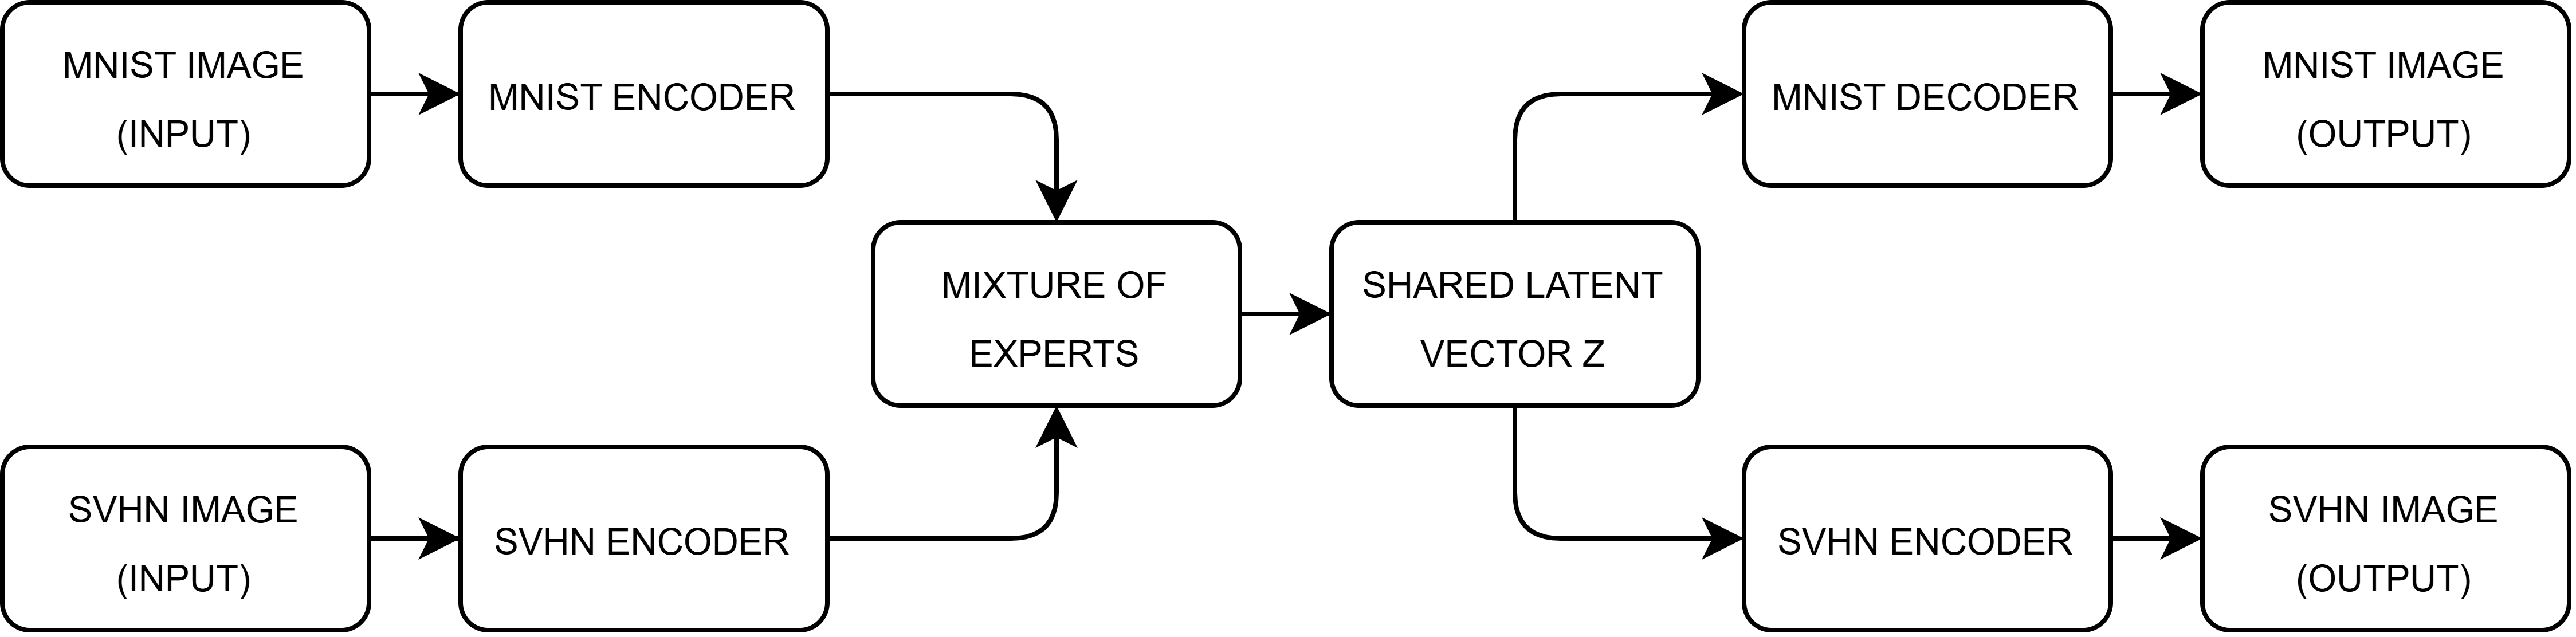
\includegraphics[width=0.8\textwidth]{diagram.png}
    \caption{Overview of the Multi-View VAE Architecture.}
    \label{fig:architecture}
\end{figure}

\section*{3.1 Image Reconstruction}
\noindent
\begin{minipage}[t]{0.38\textwidth}
    Rows 1 and 3 represent the original inputs (MNIST and SVHN), while rows 2 and 4 show their reconstructions [\ref{fig:reconstruction}]. The model handles the reconstruction of simple MNIST digits well, preserving their overall shape despite slight blurring. Sometimes model makes mistakes, such as the one with reconstructing number 2 to 3. In contrast, the reconstruction of SVHN images is heavily blurred and loses colors and background details. Overall, the model maps simple single-channel data much better than complex RGB images.
\end{minipage}\hfill%
\begin{minipage}[t]{0.58\textwidth}
    \centering
    \vspace{0pt}
    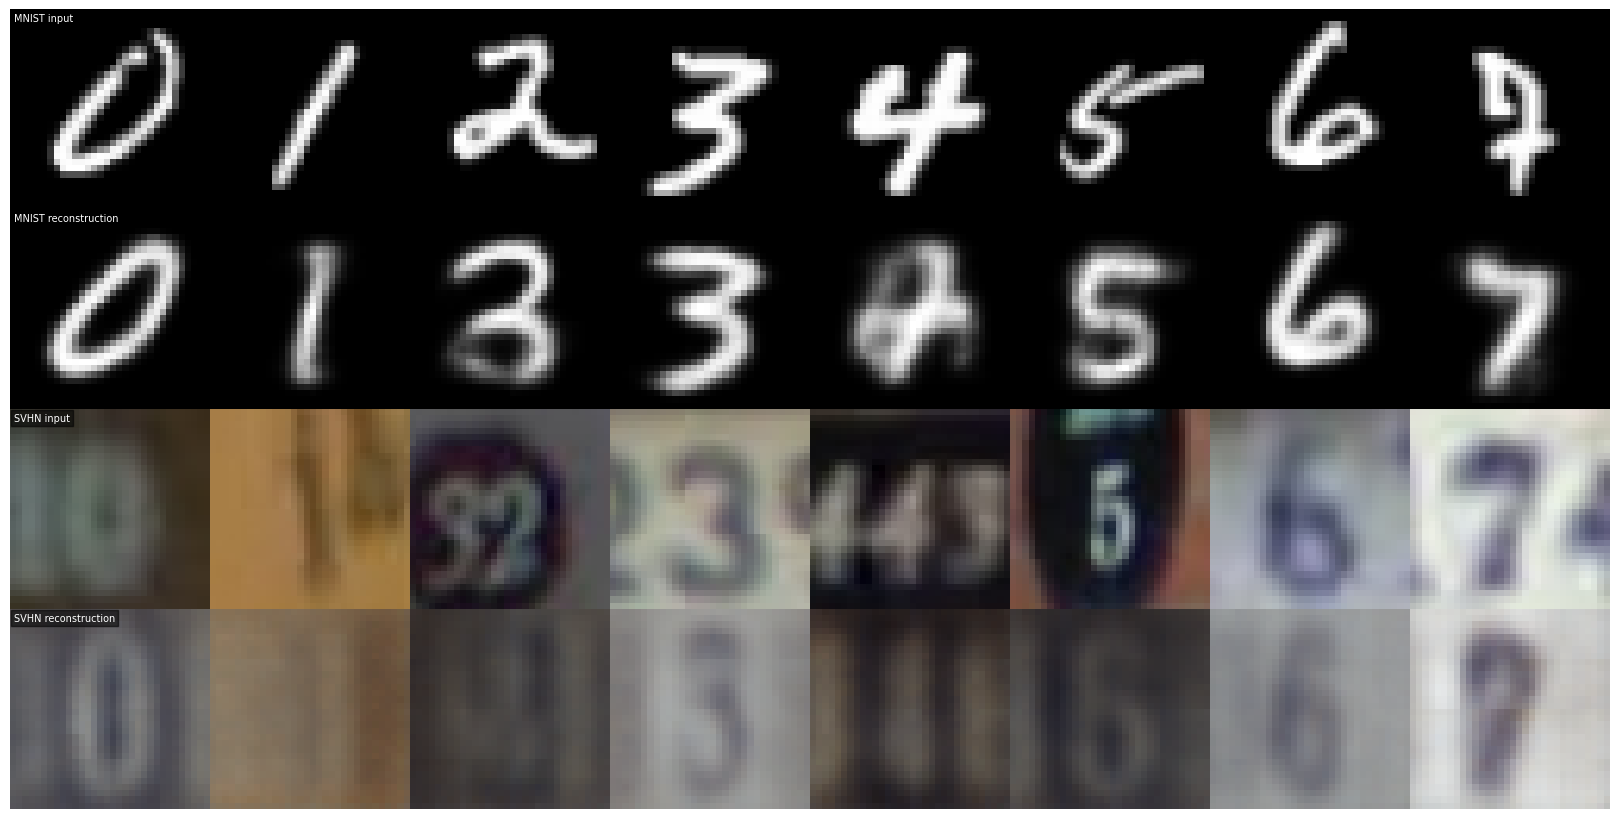
\includegraphics[width=\linewidth]{Reconstruction.png}
    \captionof{figure}{Image reconstruction results showing original inputs vs reconstructed outputs.}
    \label{fig:reconstruction}
\end{minipage}

\section*{3.2 Generation from the Prior Distribution}
\noindent
\begin{minipage}[t]{0.58\textwidth}
    \centering
    \vspace{0pt}
    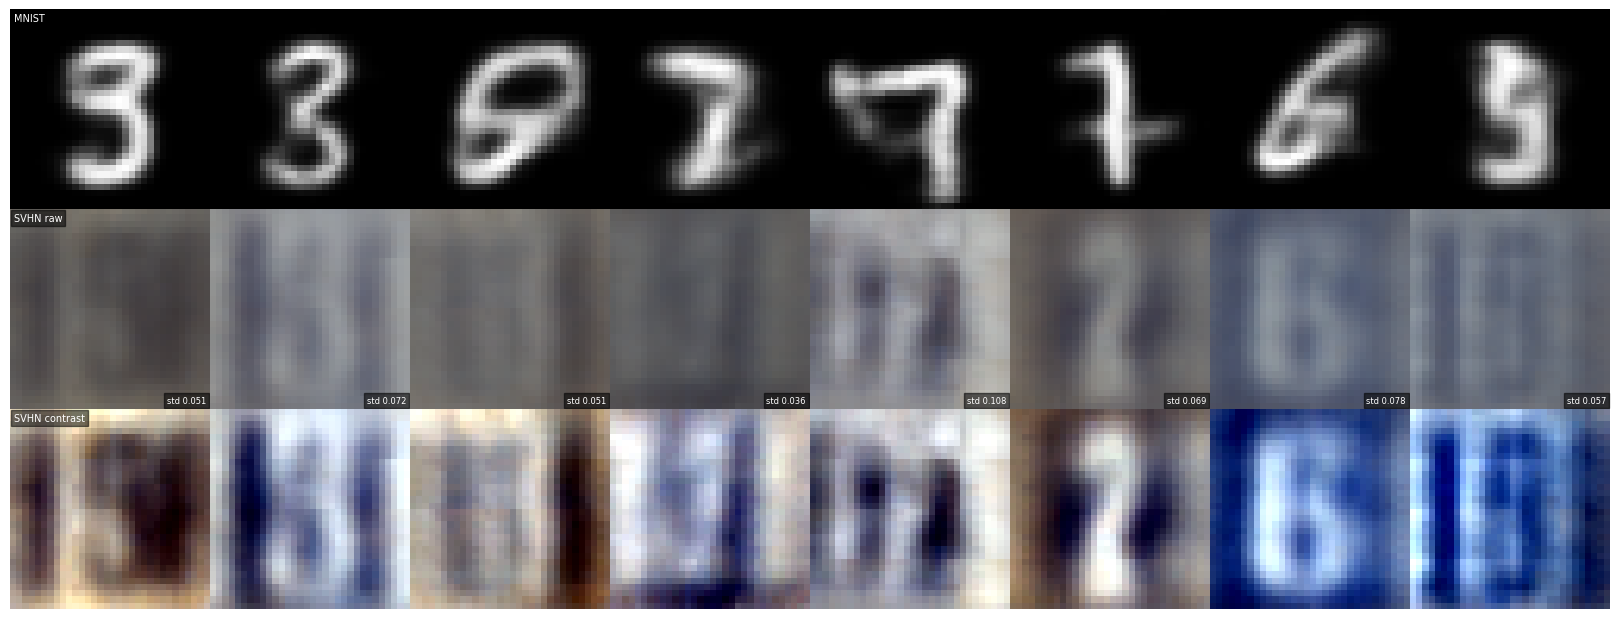
\includegraphics[width=\linewidth]{Prior.png}
    \captionof{figure}{Samples generated from prior distribution for both MNIST and SVHN domains.}
    \label{fig:prior}
\end{minipage}\hfill%
\begin{minipage}[t]{0.38\textwidth}
    \vspace{0pt}
    Rows 1 and 2 show generated MNIST and very faint SVHN samples, while row 3 displays the SVHN images with increased contrast to reveal the hidden digit outlines [\ref{fig:prior}]. Most of the digits in the row 1 actually look like the real numbers (or at least very close to them). After increasing contrast we can also see clearly that 50\% of probes matches the MNIST data. Overall, the model preserves similar shapes across both datasets despite the heavy blurring and low contrast in the SVHN view.
\end{minipage}
\section*{3.3 Cross-domain Generation}
\noindent
\begin{minipage}[t]{0.42\textwidth}
    Rows 1 through 3 show cross-domain generation from MNIST to SVHN, where row 3 displays the raw SVHN outputs (row 2) with increased contrast to reveal the translated digit outlines [\ref{fig:domain_gen}]. Without increased contrast we cannot read what is the model output, which suggests that converting grayscale images to RGB is significantly harder for the model, especially when the model needs to learn all the colored details in the background. Other than that only a few probes with increased contrast can be actually seen, but the quality of cross-domain generation is low. Rows 4 and 5 show translation from SVHN to MNIST, where the model successfully converts complex RGB inputs into clear, recognizable grayscale digits (except for two probes). Overall, the model demonstrates effective cross-domain mapping, though translating toward the SVHN domain results in very faint outputs that require contrast enhancement.
\end{minipage}\hfill%
\begin{minipage}[t]{0.54\textwidth}
    \centering
    \vspace{0pt}
    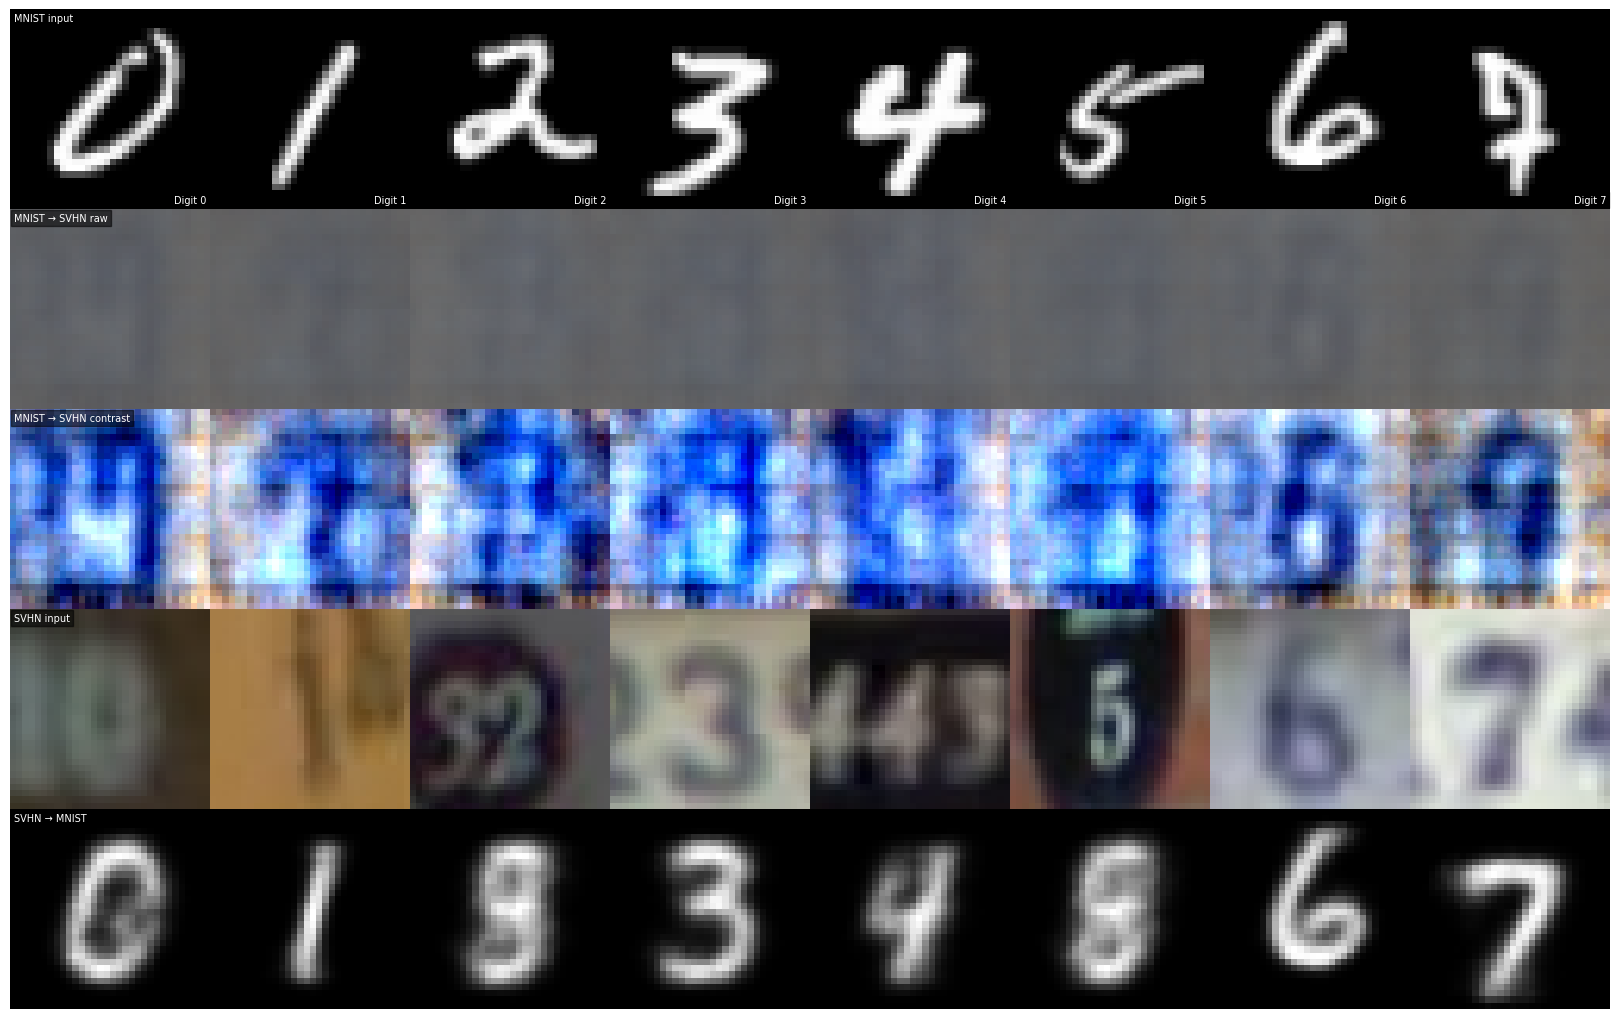
\includegraphics[width=\linewidth]{DomainGeneration.png}
    \captionof{figure}{Cross-domain generation: translating representations from MNIST to SVHN and vice versa.}
    \label{fig:domain_gen}
\end{minipage}



\subsection*{3.4 Latent Space Analysis}
\noindent
\begin{minipage}[t]{0.5\textwidth}
    \centering
    \vspace{0pt}
    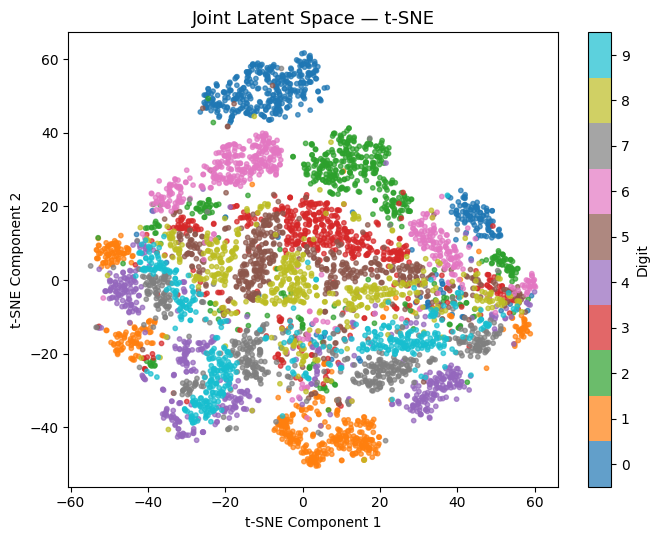
\includegraphics[width=\linewidth]{tsne.png}
    \captionof{figure}{t-SNE visualization of the Shared Latent Space.}
    \label{fig:tsne}
\end{minipage}\hfill%
\begin{minipage}[t]{0.46\textwidth}
    \vspace{0pt}
    The t-SNE visualization of the shared latent space demonstrates that the model successfully, but not perfectly clusters similar digit classes together. The representation shows consistent grouping across both domains, indicating that the shared latent space effectively aligns the multimodal features. Some digits (from 0 to 3) are more separated than the others, but on the other hand the other ones (4,5,8,9) are scattered across the entire latent space, which can lead to mistakes in cross-domain generation or prior generation.
\end{minipage}

\section*{4. Results Discussion}
The most important conclusion we can draw is that it is much easier for the model to generate MNIST images, regardless of whether this is reconstruction, cross-domain generation, or prior generation. One of the reasons for this behavior may be the complexity of SVHN images, as they include colors and different backgrounds, while MNIST is only grayscale. I tried a lot of different approaches when trying to maximize the accuracy of the MultiView VAE model, including adding warming-up epochs which increased the value of $\beta$ up to 1, exploring various latent space dimensions ranging from 20 to 128, and training the model between 20 and 40 epochs (noting that improvements became negligible after 20 epochs). Furthermore, I had to actively manipulate the loss function because the model initially failed to learn the SVHN data distribution altogether, persistently collapsing to a flat gray background. Intriguingly, although I occasionally achieved better t-SNE cluster separations in isolated runs—sometimes favoring prior generation and other times cross-domain generation—ultimately, when averaging the overall performance, this specific version yielded the best results. Consequently, this is the notebook version I decided to keep.

\end{document}